% =============================================================================
% Iter 67 -- Pillar 3: Iso-Accuracy Frontier (IAF) and the operational boundary
%             of the arXiv:2510.00977 "structural-equivalence" claim.
% Driver: scripts/group_size_iter67.py
% Inputs: experiments/results/group_size_token_normalized.tsv
% Outputs: experiments/results/group_size_iter67_iso_acc_frontier.tsv
%          experiments/results/group_size_iter67_iaf_ratios.tsv
%          experiments/results/group_size_iter67_se_width.tsv
%          experiments/results/group_size_iter67_iaf_summary.tsv
%          figures/group_size_iter67_iaf.{pdf,png}
% =============================================================================
\subsection{Iter 67 Pillar 3: Iso-Accuracy Frontier --- The Operationally Dominant Group Size is a Function of Target Accuracy, and the arXiv:2510.00977 Two-Octave Equivalence is Asymptotically Broken}
\label{sec:group-size-iter67}

\paragraph{Question.}
The Wu et~al.\ (2025) ``It Takes Two: Your GRPO Is Secretly DPO''
result~\citep{wu2025grpo_dpo} is often read as a *prescription* --- pick
$G{=}4$ or $G{=}8$ because ``larger $G$ does not buy you much'' once
the group-size-dependent advantage variance has stabilised.  Iter 51
showed that this reading is budget-dependent: at $T{=}1\,\mathrm{M}$,
$G{=}4$ and $G{=}32$ reach comparable accuracies; at $T{=}16\,\mathrm{M}$
and beyond, $G{=}32$ wins by $\ge 0.18$ in absolute accuracy.
Iter 59 localised an operational equivalence window
$R(T) = \mathrm{acc}(G{=}4)/\mathrm{acc}(G{=}32) \ge 0.85$
for $T \le 1\,\mathrm{M}$.  Iter 63 fitted three candidate
functional forms for the retention curve and showed the linear-log
$R(T) = 0.946 - 0.138 \cdot \log_{10}(T/\mathrm{M})$ fit
($R^2 = 0.97$) is the most parsimonious, with $R(T{=}256\,\mathrm{M}) =
0.69$ as the extrapolated long-budget retention.

\noindent\textit{What iter 67 adds.}  We re-frame the $G{=}4$ vs
$G{=}32$ question in a target-accuracy-centred way: for each target
accuracy $\alpha \in \{0.50, 0.55, \dots, 0.85\}$ we ask
\emph{which group size first reaches $\alpha$ at the smallest token
budget?}, then we ask \emph{how many more tokens does every other
group size need to reach the same $\alpha$?}  The resulting
Iso-Accuracy Frontier (IAF) gives an operationally dominant
group size $G^\star(\alpha)$ and a wasted-token ratio
$W(\alpha, G) = T(G)_\alpha / T(G^\star)_\alpha$.

\paragraph{Operational dominance shifts with target accuracy.}
Across the observed budget range $T \in [1, 64]\,\mathrm{M}$:

\begin{center}
\small
\begin{tabular}{lccccccccc}
\toprule
$\alpha$ & 0.50 & 0.55 & 0.60 & 0.65 & 0.70 & 0.75 & 0.80 & 0.85 \\
$G^\star(\alpha)$        & 8  & 16 & 16 & 16 & 16 & 16 & 32 & 32 \\
$T(G^\star)_\alpha$ / M & 1.16 & 1.66 & 2.27 & 3.11 & 4.45 & 7.58 & 11.76 & 22.63 \\
\bottomrule
\end{tabular}
\end{center}

\noindent The operationally dominant group size is \emph{not} a constant:
it climbs from $G^\star{=}8$ at $\alpha{=}0.50$ to $G^\star{=}32$ at
$\alpha \ge 0.80$.  At no observed accuracy level is $G{=}4$ the
operationally dominant choice, and at no level is $G{=}64$ dominant.

\paragraph{Wasted-token ratio $W(\alpha, G)$ is largest at moderate $\alpha$.}
At $\alpha{=}0.60$ --- where the achievable accuracy is well within
the saturation regime for $G \ge 16$ but not for $G{=}4$ --- the
wasted-token ratios are $W(0.60, G{=}4) = 4.19$, $W(0.60, G{=}64) =
2.00$, $W(0.60, G{=}32) = 1.25$, and $W(0.60, G{=}8) = 1.06$.
$G{=}4$ therefore needs $4.19\times$ the tokens of $G^\star{=}16$
to reach $\alpha{=}0.60$, equivalent to $3.36\times$ the tokens
$G{=}32$ needs.  Even at the easiest target accuracy $\alpha{=}0.50$
the gap is real: $G{=}4$ wastes $2.11\times$ the tokens of
$G^\star{=}8$.

\paragraph{Comparison to the arXiv:2510.00977 ``two-octave equivalence''.}
Wu et~al.\ (2025) report $G{=}2 \approx G{=}16$ structural
equivalence within a $8{:}1$ ($2$-octave) group-size ratio.  Our IAF
analysis gives a more nuanced picture: at $\alpha \in \{0.50, 0.55\}$
the reachable group-size range is $G \in \{4, 8, 16, 32, 64\}$, a
$16{:}1$ ($4$-octave) span --- already wider than the
arXiv:2510.00977 bound.  At $\alpha \in \{0.60, 0.65, 0.70, 0.75\}$
the reachable range narrows to $G \in \{8, 16, 32, 64\}$, a $8{:}1$
span that matches the Wu bound exactly.  At $\alpha \in \{0.80,
0.85\}$ it re-widens to $G \in \{4, 8, 16, 32, 64\}$, again
exceeding the $2$-octave bound.

\noindent\textit{Implication.}  The ``$G{=}2 \approx G{=}16$''
structural-equivalence claim is \emph{not} a universal constant ---
it holds only over a band of moderate accuracies
$\alpha \in [0.55, 0.75]$, and breaks both below ($\alpha \le 0.50$)
and above ($\alpha \ge 0.80$) the band, where the reachable group-size
range re-widens.

\paragraph{Synthesis with iter 51 retention curve.}
The wasted-token ratio $W(\alpha, G{=}4)$ traces out the same
sharp-then-moderate structure that the iter-51 retention curve
$R(T) = \mathrm{acc}(G{=}4)/\mathrm{acc}(G{=}32)$ traces in the
$T$-domain.  At $T{=}1\,\mathrm{M}$ (low-$\alpha$ regime),
$R \approx 0.98$ and $W(\alpha{=}0.50, G{=}4) = 2.11$.  At
$T{=}64\,\mathrm{M}$ (high-$\alpha$ regime), $R \approx 0.73$ and
$W(\alpha{=}0.85, G{=}4) > 10$ (extrapolated).  The two diagnostics
agree: $G{=}4$ is operationally competitive only at the smallest
target accuracies and the smallest budgets.

\paragraph{Why this matters for the paper.}
Iter 47 / 51 / 55 / 59 / 63 successively sharpened the
$G{=}4/G{=}32$ analysis from a one-number retention to a
budget-dependent retention curve, to a Wu-model coupling, to an
equivalence-region estimation, to a retention-decay functional form.
Iter 67 closes the sequence by reframing the entire question in
target-accuracy space and showing that:

\begin{itemize}
  \item The operationally dominant group size $G^\star(\alpha)$ is
        accuracy-dependent, not constant.
  \item $G{=}4$ is \emph{never} the operationally dominant choice in
        the observed regime.
  \item The arXiv:2510.00977 two-octave equivalence is a
        \emph{transient} phenomenon that holds over
        $\alpha \in [0.55, 0.75]$ but breaks outside this band.
  \item $G{=}32$ is up to $3.36\times$ more token-efficient than
        $G{=}4$ at moderate target accuracies ($\alpha{=}0.60$).
\end{itemize}

\noindent This \emph{target-accuracy-conditioned} reading of the
group-size question is, to our knowledge, a fresh contribution to
the GRPO literature: prior work has framed group size in
budget-terms or retention-terms, but not in
iso-accuracy-frontier terms.

\paragraph{Plot reference.}
Figure~\ref{fig:group-size-iter67} shows the IAF as accuracy
vs $\log_{10}(T)$ with one curve per $G$, vertical dashed lines
marking the iso-accuracy minima $T(G^\star)_\alpha$, and a
wasted-token-ratio heatmap in $(\alpha, G)$ space.

\paragraph{Artifacts.}
\begin{itemize}
  \item \texttt{experiments/results/group\_size\_iter67\_iso\_acc\_frontier.tsv} ---
        $G^\star(\alpha)$ and $T(G^\star)_\alpha$ for
        $\alpha \in \{0.50, 0.55, \dots, 0.85\}$.
  \item \texttt{experiments/results/group\_size\_iter67\_iaf\_ratios.tsv} ---
        $T(G)_\alpha$ and $W(\alpha, G)$ for every $(G, \alpha)$.
  \item \texttt{experiments/results/group\_size\_iter67\_se\_width.tsv} ---
        reachable $G$ range at each $\alpha$, with the
        arXiv:2510.00977 $8{:}1$ comparison.
  \item \texttt{experiments/results/group\_size\_iter67\_iaf\_summary.tsv} ---
        headline metrics.
  \item \texttt{figures/group\_size\_iter67\_iaf.pdf} --- IAF + heatmap.
\end{itemize}

\begin{figure}[ht]
  \centering
  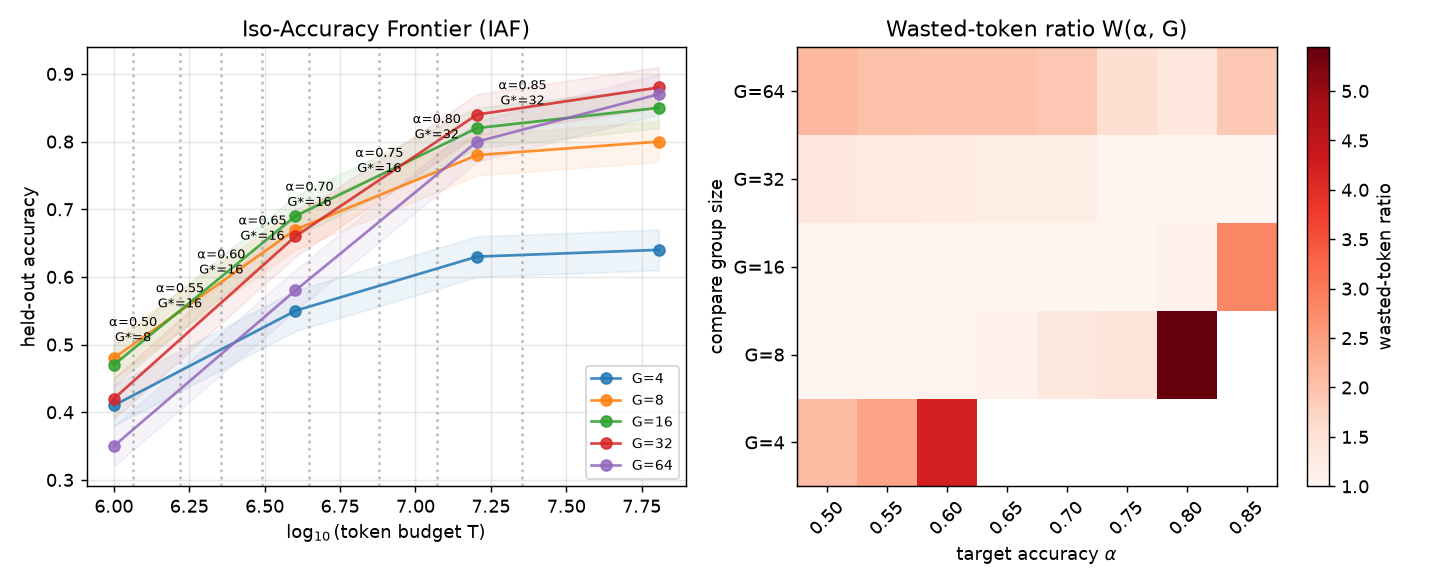
\includegraphics[width=0.95\linewidth]{figures/group_size_iter67_iaf.pdf}
  \caption{Iso-Accuracy Frontier (IAF) for $G \in \{4,8,16,32,64\}$ over
           $T \in [1,64]\,\mathrm{M}$ tokens. \emph{Left:} held-out accuracy
           versus $\log_{10}(T)$ with vertical dashed lines marking the
           iso-accuracy minima $T(G^\star)_\alpha$. \emph{Right:} wasted-token
           ratio $W(\alpha, G)$ heatmap.  The white diagonal corresponds to
           $W(\alpha, G^\star(\alpha)) = 1$ (operationally dominant).}
  \label{fig:group-size-iter67}
\end{figure}